\lettrine{C}{loud} computing has reshaped how companies build software, shifting the focus to scalable solutions that leverage elastic infrastructure. 
Applications are increasingly containerized and managed with platforms such as Kubernetes, while serverless computing has also gained traction.  

\vspace{0.5em} Being inherently distributed, cloud-native systems face the challenges outlined by the CAP theorem: architects must balance Partition Tolerance, Consistency, and Availability. 
This has led to designs that relax strong consistency in favor of availability through Eventual Consistency.  

\begin{boxF}
    The CAP theorem \cite{c1} states that, in the presence of a network partition, a system must trade off between Consistency and Availability. 
    Eventual Consistency aligns with PA (Partition Tolerance and Availability), allowing a system to remain responsive during partitions while deferring full consistency until recovery. 
\end{boxF}

\begin{figure}[h]
    \centering
    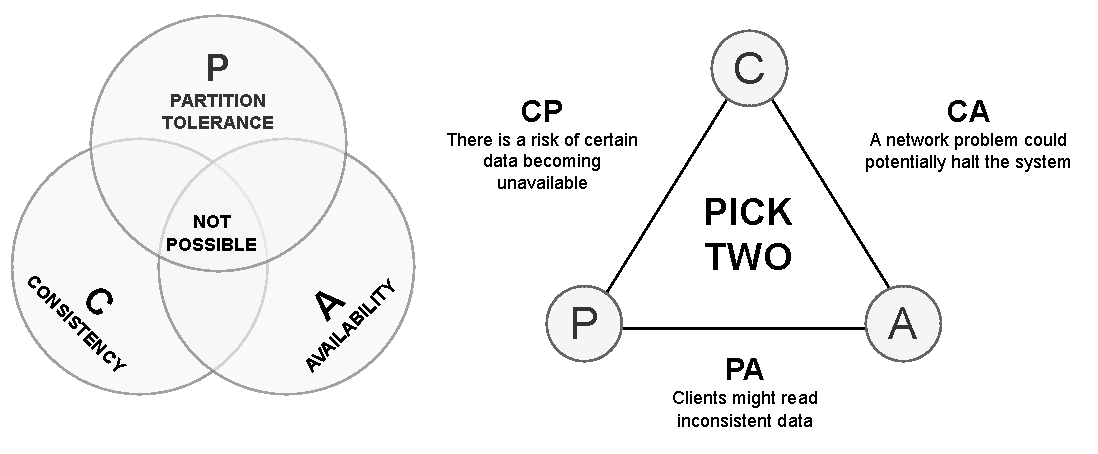
\includegraphics[width=\linewidth]{introduction/cap-theorem.pdf}
    \caption{CAP Theorem}
    \label{fig:cap-theorem}
\end{figure}

Another major trend is the adoption of asynchronous patterns and event-streaming frameworks such as Apache Kafka, which handle continuous flows of events without a clear beginning or end.  
In this setting, orchestration has proven complex and difficult to scale, whereas choreography-based systems often provide better scalability.  

Figure \ref{fig:cloud-architecture} shows a typical cloud architecture: clients authenticate with a centralized Identity Provider, which issues a token subsequently used to access server resources. 
Two widely adopted protocols here are OpenID \cite{c4} for authentication and OAuth \cite{c5} for authorization.  

\begin{figure*}[htbp]
    \centering
    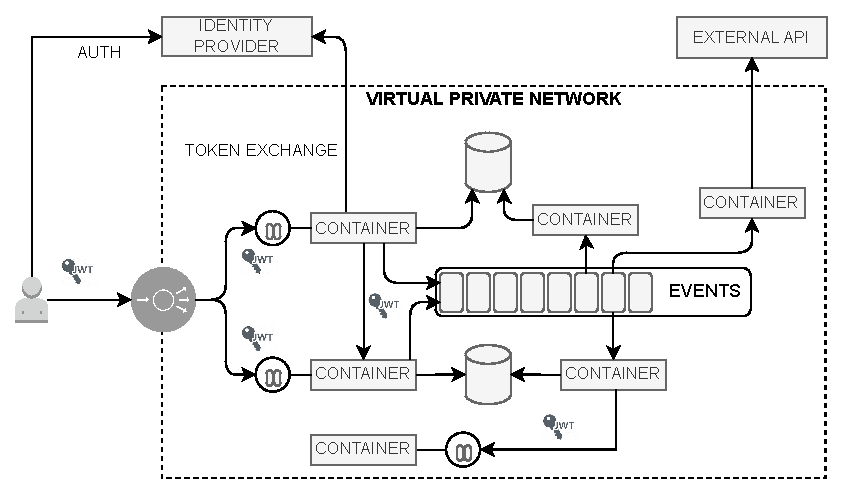
\includegraphics[width=0.7\textwidth]{introduction/cloud-architecture.pdf}
    \caption{Cloud Architecture}
    \label{fig:cloud-architecture}
\end{figure*}

\vspace{0.5em} Within these protocols, JSON Web Tokens (JWT) \cite{c6} have become central. 
Compact and digitally signed, they ensure message integrity and enable secure communication between client and server.  

\vspace{0.5em} Access control remains a critical concern. Models such as Role-Based Access Control (RBAC) and Attribute-Based Access Control (ABAC) have paved the way for Policy-Based Access Control (PBAC) \cite{c7}.  

\vspace{0.5em} A further challenge arises in transport-layer communication, for example with Kafka and stream-processing systems, where it is not always feasible to propagate a token.

\begin{figure}[htbp]
    \centering
    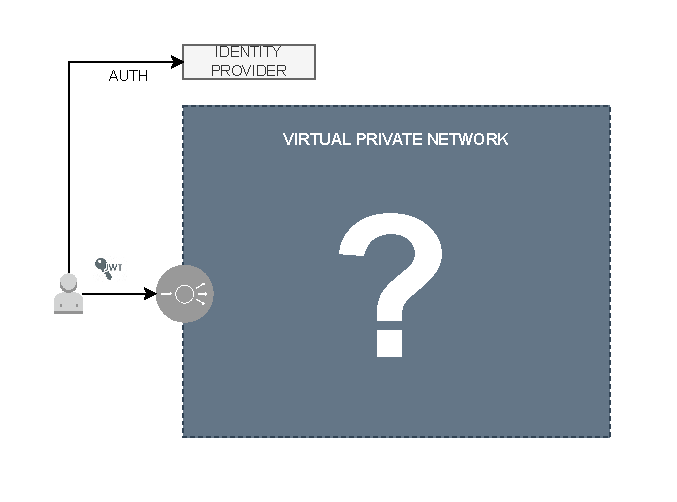
\includegraphics[width=0.5\textwidth]{introduction/current-model.pdf}
    \caption{Building inside a Perimeter}
    \label{fig:current-model}
\end{figure}

\vspace{0.5em} This exposes a key limitation of the current model: it works at the perimeter, where tokens are validated at delivery, but what happens inside the enterprise afterward is not standardized. 
Authorization is essentially assumed to remain valid once accepted at the boundary, and the system continues to treat it as true for the rest of the time.  
While this trade-off was once acceptable, it cannot be sustained in environments that must support AI agents.  

Moreover, modern distributed systems increasingly operate \emph{without clear perimeters}. 
In cloud-native, multi-tenant, and hybrid environments, workloads, services, and agents continuously interact across organizational and network boundaries. 
In such scenarios, the very assumption of a fixed perimeter for validation no longer holds, making token-based authorization even more fragile.  

It follows that the current model is not suitable for AI agents, which require dynamic, context-aware, and continuously validated authorization. 
The goal is not to replace existing protocols but to complement them, addressing the gaps they have historically overlooked.
